\documentclass[../../DD.tex]{subfiles}
\begin{document}
\section{P-IDM}
	The landmarks of the website are composed by the introductory pages of all the kinds of topic, in addition to both the single topics and the \textit{Home Page}. From the \textit{Home Page} it's possible to reach also the very next \textit{Event}.
	\newline
	All the introductory pages use an index pattern to link the single pages of their group. For \textit{Person}, \textit{Event} and \textit{Course} kinds of topic, this is the only way to navigate among their elements. \textit{Musical Instruments}, instead, are linked to the related instruments by an all-to-all pattern: each one has a direct link to all its related \textit{Musical Instrument}.
	\newline
	\textit{Contacts} topic is divided into two different pages (or tabs) linked with an all-to-all pattern (they are simply linked together): the first one contains \textit{Contacts} with \textit{Social channels}, the other one \textit{Where we are}.
	\newline
	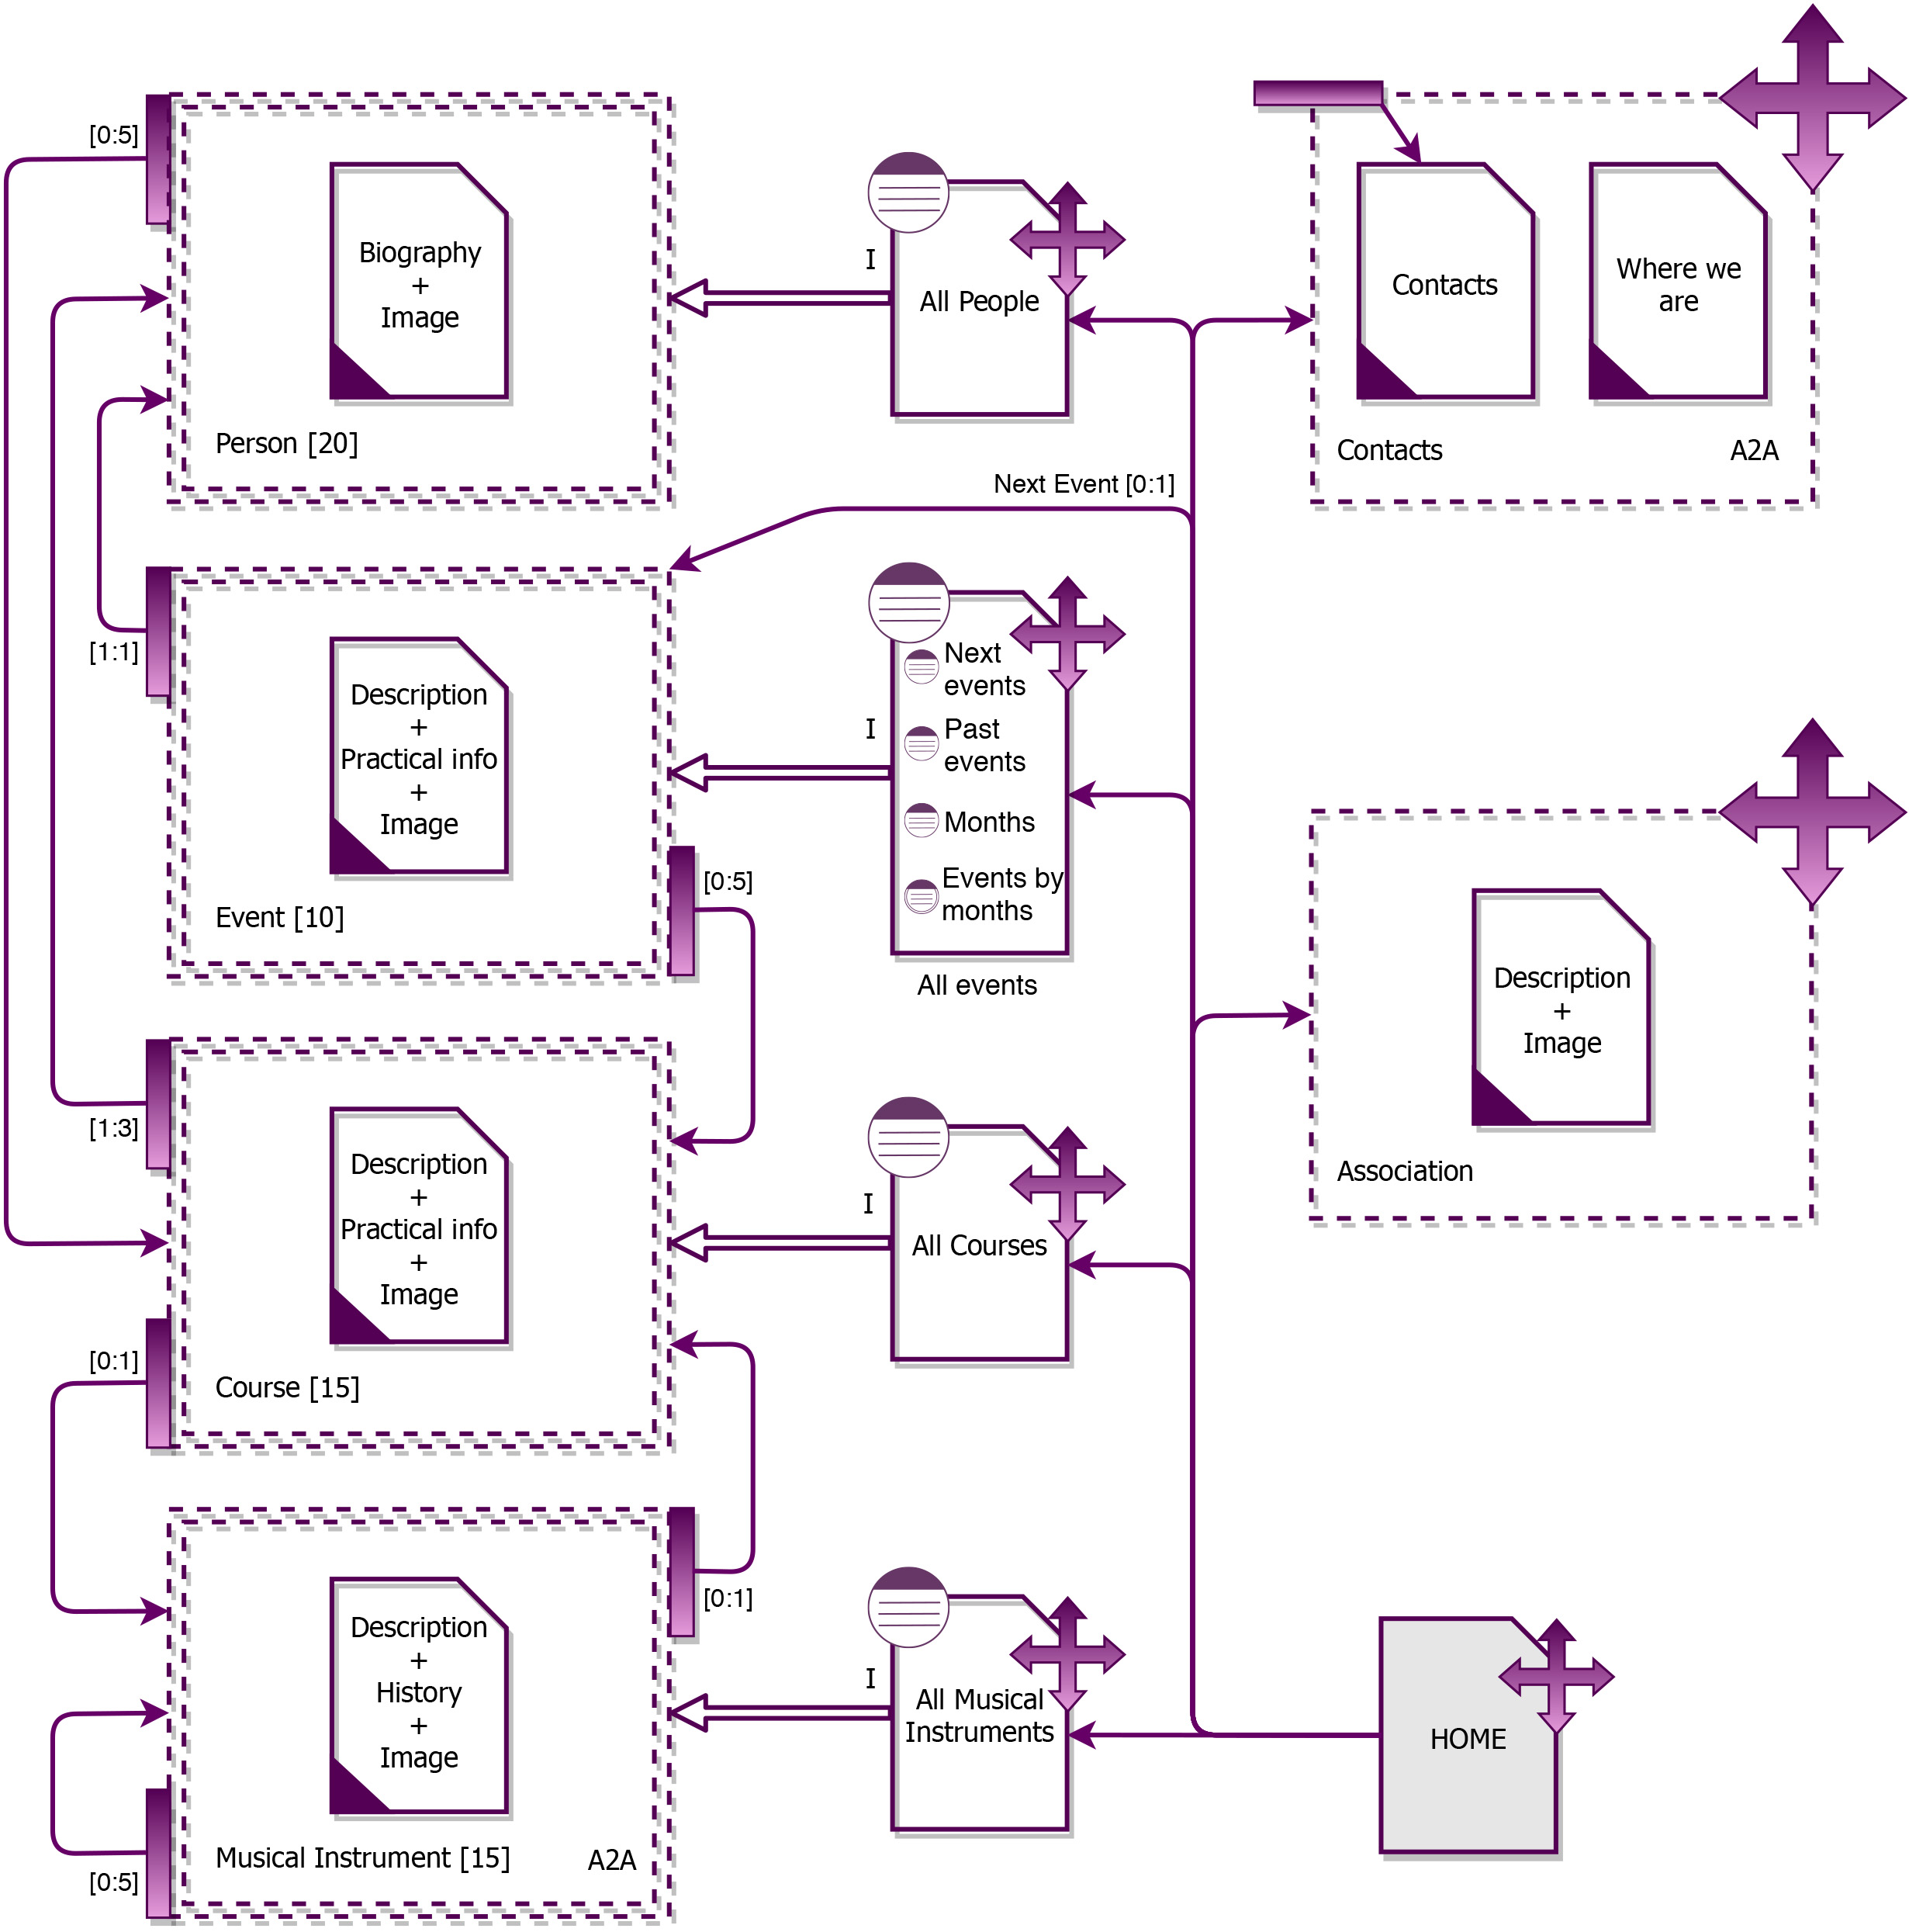
\includegraphics[width=\textwidth,height=\textheight,keepaspectratio]{IDM/P-IDM.jpg}
\end{document}
